\documentclass[../rapport_MVEX01-11-05]{subfiles}
\begin{document}
Resultat

Klassificering av gester med hjälp av kNN

Den största andelen korrekt klassificerade gester vi lyckades uppnå
var 91,5\%. Denna procent uppnåddes då samtliga gester var
inkluderade, antalet aktiverade egenskaper var 10 och värdet på $k$
i kNN-metoden var 7. Egenskaperna som användes var det första,
andra, tredje och sjunde Hu-momentet, centroidens position i den
inneslutande lådan, fyrkantighet, soliditet, excentricitet,
konvexitet och utsträckning. Följande plot visar hur andelen
korrekta klassficeringar beror på antalet aktiverade egenskaper och
värdet på $k$:

(PLOT)

Det framgår tydligt att antalet aktiverade egenskaper har stor
inverkan på resultatet då man använder sig av färre än
5st. Därefter planar procenttalet ut för att återigen stiga då
fler än 10 egenskaper används. Andelen korrekta klassificeringar
ökar också i takt med att $k$ ökar från 1 till 7, för att sedan
bidra negativt då värdet ökar från 7 till 13. Med det optimala
valet av egenskaper och $k$ blev prestandan för respektive gest

(PLOT)

(Inkludera resultat där problemgester är borttagna?)

(i ordning: det tredje Hu-momentet, det andra Hu-momentet, centroidens
y-position i den inneslutande lådan, fyrkantighet, soliditet,
excentricitet, konvexitet, första Hu-momentet, utsträckning och det
sjunde Hu-momentet.) 

\subsection{\knn}

\begin{table}
	  \centering
		\label{tab:tolkningsmatris}
		\caption{}
    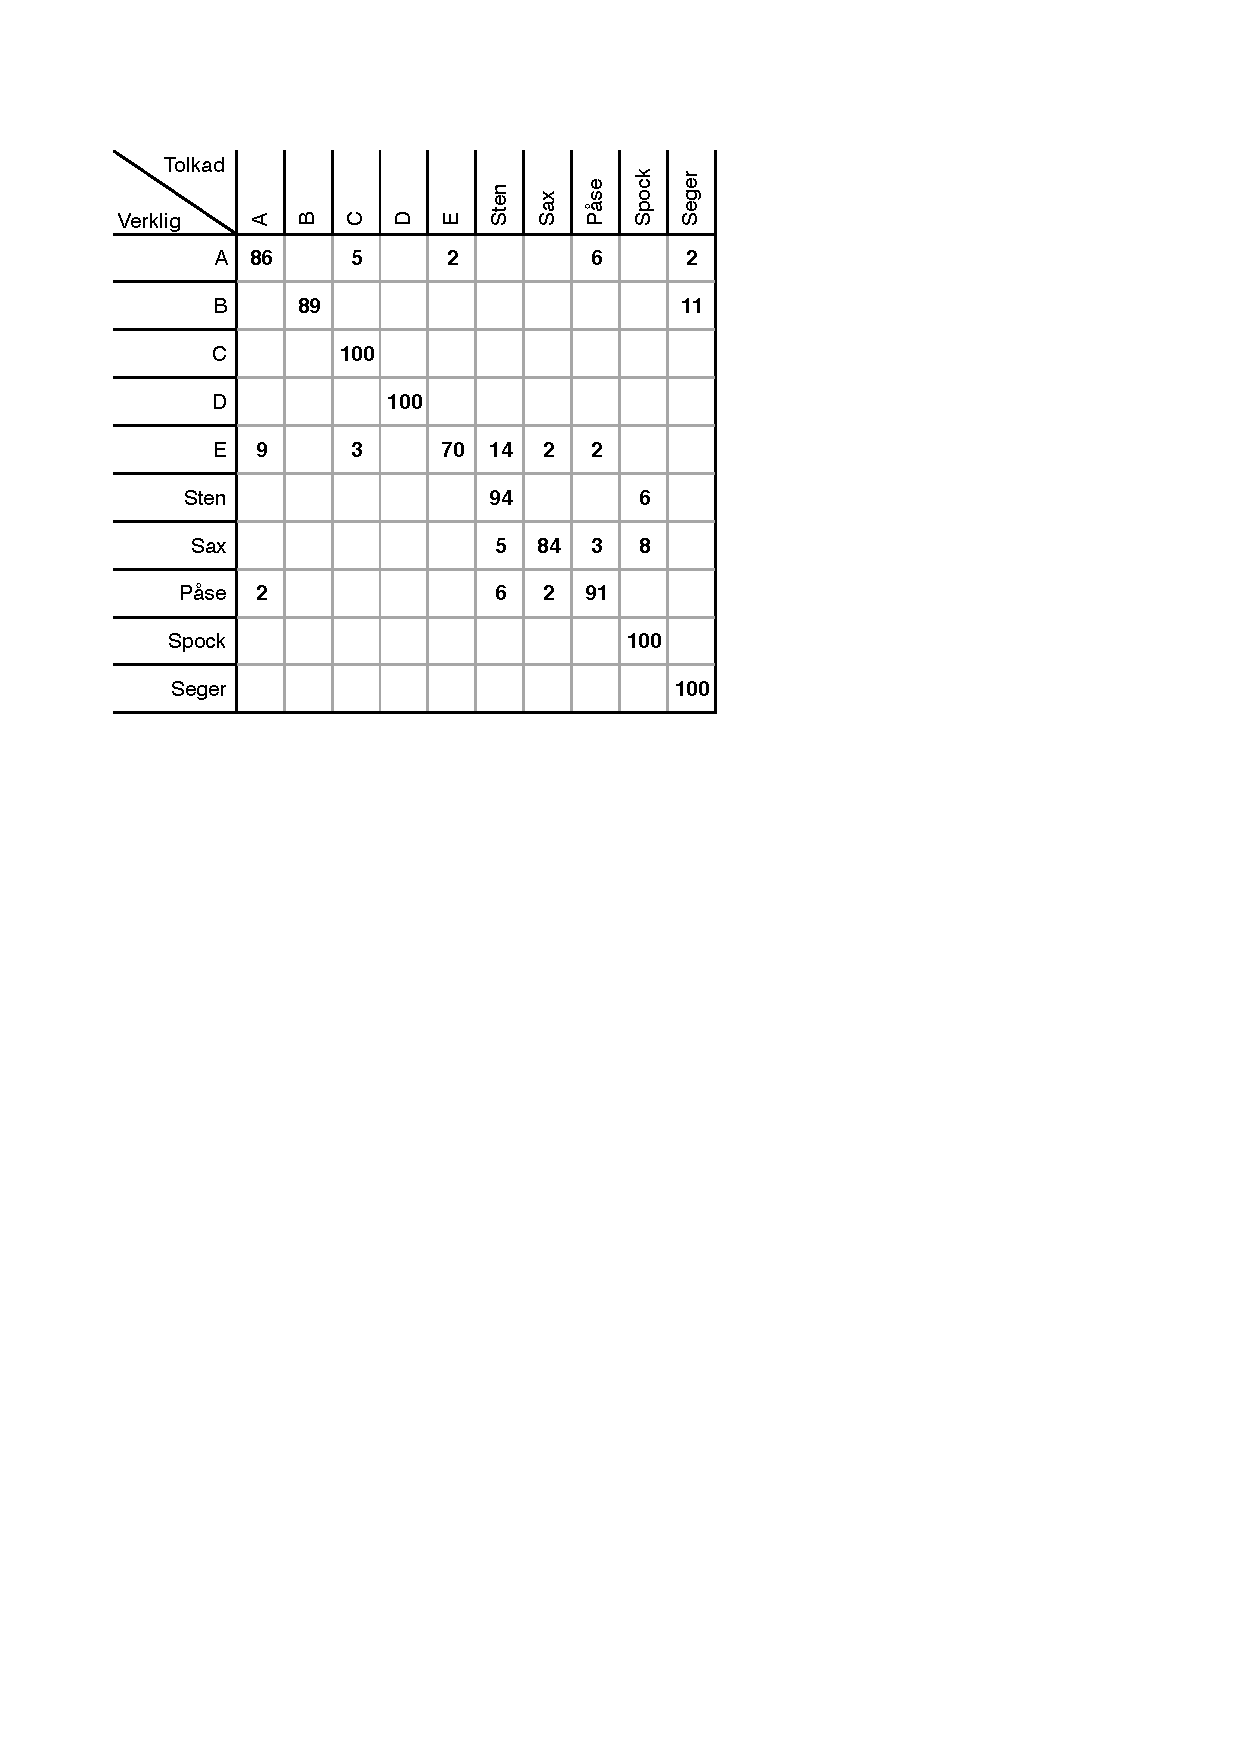
\includegraphics[trim=0 0 0 2.5cm]{bilder/tolkningsmatris.pdf}
		%\begin{tabular}{l|cccccccccc}
		%\backslashbox{Verklig}{Tolkad} & a & b & c & d & e & Sten & Sax & Påse & Spock & Seger\\
		%\toprule
		%a & 86 &  & 5 &  & 2 &  &  & 6 &  & 2 \\ 
		%b &  & 89 &  &  &  &  &  &  &  & 11 \\ 
		%c & &  & 100 &  &  &  &  &  &  &  \\ 
		%d &  &  &  & 100 &  &  &  &  &  &  \\ 
		%e & 9 &  & 3 &  & 70 & 14 & 2 & 2 &  &  \\ 
		%Sten & &  &  &  &  & 94 &  &  & 6 &  \\ 
		%Sax & &  &  &  &  & 5 & 84 & 3 & 8 &  \\ 
		%Påse & 2 &  &  &  &  & 6 & 2 & 91 &  &  \\ 
		%Spock &  &  &  &  &  &  &  &  & 100 &  \\ 
		%Seger & &  &  &  &  &  &  &  &  & 100 \\  
		%\end{tabular}
		
\end{table}

%\notes{Jag vill ha den som \LaTeX{} men inte som en ''ful'' tabell. Det verkar
%finnas ett paket \texttt{slashbox} som gör den sneda biten, i komination med
%typ \texttt{colortbl} kan det bli hyfsat okej. Men riktiga tabeller ska vi nog
%använda \texttt{booktabs till}.}

\end{document}
